\section{ClickNP Elements}
\label{clicknp:sec:elements}

In this section, we present the Line Of Code (LOC) (excluding the host program) and resource utilization of some common elements under reasonable parameter settings.

All elements discussed in this section can process a 40 Gbps line rate for all Ethernet packet sizes under a 190 MHz clock rate, i.e., one cycle per iteration for elements processing packet flits, and up to 3 cycles per iteration for elements processing metadata only.

\subsection{Basic Connectors}

\begin{table}[h!]
	\centering
	\label{clicknp:tab:Basic Connectors}
	\begin{tabular}{l|r|r|r}
		Element & LOC & Logic & Memory \\
		\hline
		Tee	&  & \%  & 0\% \\
		Mux	&  & \% & 0\% \\
		Demux & & \% & 0\% \\
		FlitMux & & \% & 0\% \\
		FlitDemux & & \% & 0\% \\
	\end{tabular}
\end{table}


\subsection{Programmable Header Parser}

The packet parser is a crucial component of the network processor, with its complexity arising from tunneling protocols and the diversity of protocols in each layer.

The uncertainty of outer layers introduces a non-constant header offset in the packet. For instance, an Ethernet packet without VLAN has an IP header offset of 14, while an Ethernet packet with VLAN has an IP header offset of 18. Simply using a variable as an index to the packet byte array is highly inefficient in OpenCL. An array with one or more variable index access will be implemented as block SRAM in FPGA, which only supports one read operation per cycle. To parse the packet header (which includes many array accesses) in one cycle, we need to implement the packet buffer as a register in FPGA, which requires all accesses to the packet buffer array to have a constant index.

%If we create an element for each packet header, then each element needs to shift the packet payload in order to ``peel off'' the parsed header. The first drawback is that each element introduces some overhead in logic utilization. Since there are multiple leaf elements representing the innermost header to parse, and different elements have different latencies, output packets at the final mux will be out-of-order. The reordering buffer would take considerable local memory. Furthermore, in the case of network virtualization and tunneled protocols, there will be a loop of elements that each tunneled packet would travel twice, which lowers throughput of packet parser.

To implement a packet parser with all packet buffer offsets to be constant, without shifting packet payload after each header is parsed, we need to enumerate all possible parsing paths (e.g. Ethernet $\rightarrow$ IP, Ethernet $\rightarrow$ VLAN $\rightarrow$ IP), duplicate parser code for each path and calculate offset for each access to packet buffer. Doing such work manually is frustrating and error-prone, therefore ClickNP provides a general \textit{.state\_machine} abstraction, which can generate a decision tree composed of all possible state migration paths and calculate all packet buffer offsets at compilation time.

\begin{lstlisting}
.state_machine {
    constexpr offset = 0;
    .parser_define MAX_STATE_REPEAT 2;
    begin {
        constexpr offset += 12;
        ushort next_proto = *(ushort *) &input[offset];
        constexpr offset += 2;
        if (next_proto == PROTO_VLAN)
            .goto_state VLAN;
        else if (next_proto == PROTO_IPv4)
            .goto_state IPv4;
        else
            .goto_state end;
    }
    VLAN {
        if (!meta.vlan)
            meta.vlan = *(ushort *) input[offset];
        ushort next_proto = *(ushort *) &input[offset + 2];
        constexpr offset += 4;
        if (next_proto == 0x8100)
            .goto_state VLAN;
        else if (next_proto == 0x0800)
            .goto_state IPv4;
        else
            .goto_state end;
    }
    IPv4 {
        .if (STATE_REPEAT == 1) {
            meta.src_ip = *(uint *) &input[offset + 12];
            meta.dst_ip = *(uint *) &input[offset + 16];
        } .else {
            meta.inner_src_ip = *(uint *) &input[offset + 12];
            meta.inner_dst_ip = *(uint *) &input[offset + 16];
        }
        ushort next_proto = input[offset + 9];
        constexpr offset += 20;
        if (next_proto == 94)
            .goto_state IPv4; // IP-in-IP
        else if (next_proto == 97)
            .goto_state begin; // ETHERIP
        else
            .goto_state end;
    }
}
\end{lstlisting}


\begin{figure}[!t]
	\centering
	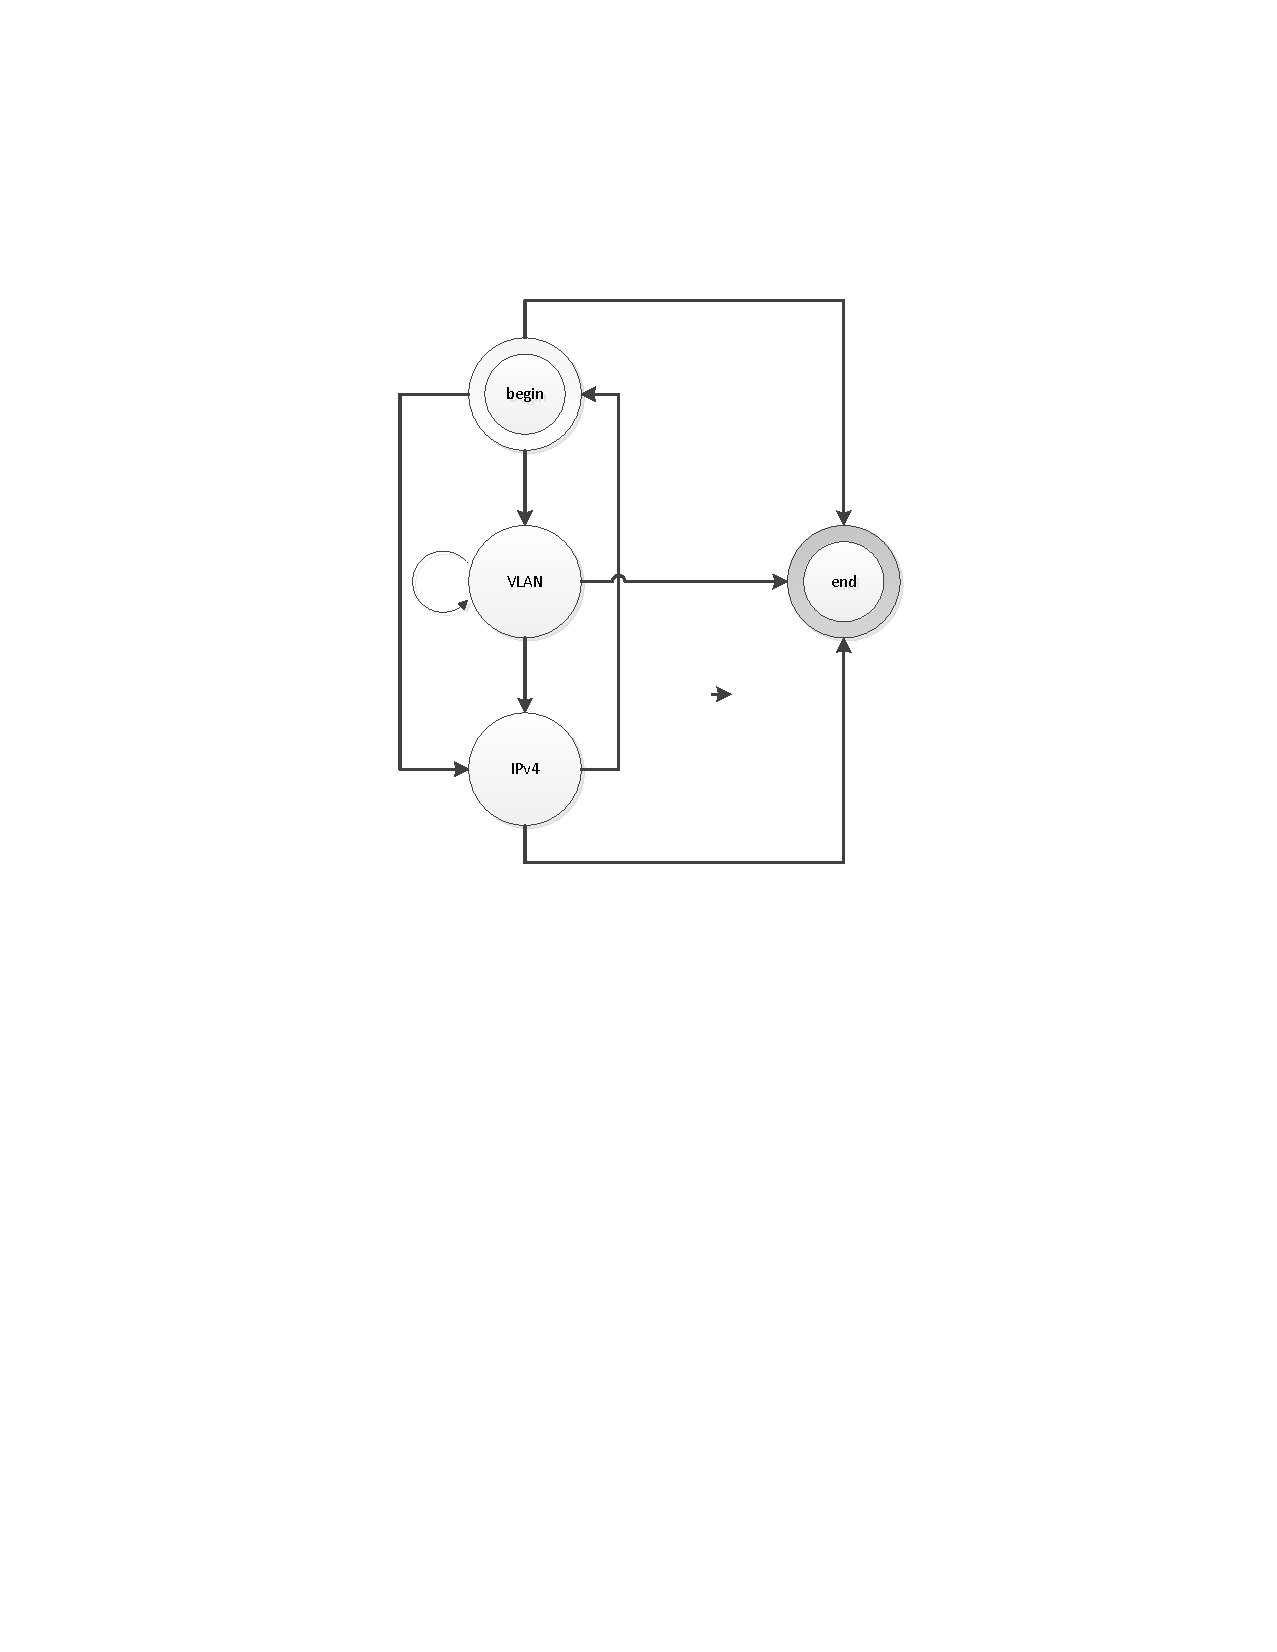
\includegraphics[width=0.7\columnwidth]{image/StateMachine}
	\vspace{-0.15in}
	\caption{Sample State Machine for Header Parser}
	\vspace{-0.15in}
	\label{clicknp:fig:StateMachine}
	%    
\end{figure}

The code above implements a sample header parser as illustrated in figure \ref{clicknp:fig:StateMachine}, where each state is set to repeat a maximum of two times. From 44 lines of code with 3 states, it generates 314 lines of code with 27 states, consuming only 2\% of the logic resource.

Below are some parsers designed to extract metadata from some well-known protocols. The code for these elements can be easily modified to extract new fields or incorporate new protocols.

\begin{table}[h!]
	\centering
	\label{clicknp:tab:PacketParsers}
	\begin{tabular}{l|r|r|r}
		Element & LOC & Logic & Memory \\
		\hline
		EthVlanParser & & \% & \% \\
		IPv4\_Parser & & \% & \% \\
		IPv6\_Parser & & \% & \% \\
		FlowTuple\_Parser & & \% & \% \\
		TCP\_Parser & & \% & \% \\
		NVGRE\_Parser & & \% & \% \\
		VXLAN\_Parser & & \% & \% \\
	\end{tabular}
\end{table}

\subsection{Lookup Tables}
\label{clicknp:subsec:lookuptables}

The \textit{HashTable} is implemented using Cuckoo hash \cite{pagh2004cuckoo} with two memory banks, which can be used for exact matching.

\begin{figure}[h!]
	\centering
	
\includegraphics[width=0.6\columnwidth]{image/logo}
	\vspace{-0.15in}
	\caption{HashTable Collision Rate, x: occupancy, y: hash collision rate, lines: sequential IP, sequential port, random, theory}
	\vspace{-0.15in}
	\label{clicknp:fig:HashTableCollisionRate}
	%    
\end{figure}

The \textit{TCAM} compares all entries in parallel and finds the lowest entry index that matches. Due to the high logic resource utilization of TCAMs, we designed the \textit{HashTCAM} to balance logic with memory. This design is based on the observation that bit-mask patterns in a set of real-world wildcard rules are limited. To reduce the bit width of the match key, commodity switching chips require users to specify bit-mask patterns before rule insertion. For example, Broadcom Trident II \cite{broadcomethernet} only supports 16 bit-mask patterns.

HashTCAM also imposes a limitation on the number of bit-mask patterns. For each unique bit-mask pattern, HashTCAM allocates a HashTable and fills its mask field. All rules sharing this bit-mask pattern can be inserted into the HashTable, where the key is the masked original key and the value is the index in the original TCAM. Match results from HashTables are arbitrated to find the lowest index (highest priority) and get the match result by index from SRAM. The \textit{HashTCAM} class in the host program provides a TCAM-like interface to abstract away HashTable allocation, rule update, and SRAM update.

I'm sorry, but you didn't provide any LaTeX content to translate. Please provide the content you want to translate.
